\documentclass[13pt,a4paper]{article}
\usepackage[utf8]{vietnam}
\usepackage{amsmath}
\usepackage{amsfonts}
\usepackage{amssymb}

\usepackage[left=3.00cm, right=2.00cm, top=2.00cm, bottom=2.00cm]{geometry}
\usepackage{mathptmx}
\usepackage{graphicx}
\usepackage{float}
\usepackage{tikz}
\usetikzlibrary{calc}
\usepackage{indentfirst} %thu vien thut dau dong
\renewcommand{\baselinestretch}{1.2}% Gian dong 1.2
\setlength{\parskip}{6pt} %spacing after
\setlength{\parindent}{1cm} %thut dau dong moi doan
\usepackage{titlesec}
\titlespacing*{\section}{0pt}{0pt}{30pt} %Heading 1
\titleformat*{\section}{\fontsize{16pt}{0pt}\selectfont \bfseries \centering}

\titlespacing*{\subsection}{0pt}{10pt}{0pt} %Heading 2
\titleformat*{\subsection}{\fontsize{14pt}{0pt}\selectfont \bfseries}

\titlespacing*{\subsubsection}{0pt}{10pt}{0pt} %Heading 3
\titleformat*{\subsubsection}{\fontsize{13pt}{0pt}\selectfont \bfseries \itshape}

\titlespacing*{\paragraph}{0pt}{10pt}{0pt} %Heading 4
\titleformat*{\paragraph}{\fontsize{13pt}{0pt}\selectfont \itshape}

\begin{document}
\begin{titlepage}

\begin{center}
\vspace{-6pt} TRƯỜNG ĐẠI HỌC BÁCH KHOA THÀNH PHỐ HỒ CHÍ MINH\\
\textbf{\fontsize{16pt}{0pt}\selectfont BỘ MÔN VIỄN THÔNG}
\vspace{0.5cm}
\begin{figure}[H]
	\centering
	
\includegraphics[scale=.30]{image/bachkhoa.png}
\end{figure}
\vspace{0.5cm}
\fontsize{24pt}{0pt}\selectfont BÁO CÁO\\
\vspace{12pt}
\textbf{\fontsize{32pt}{0pt}\selectfont THỰC TẬP TỐT NGHIỆP}
\vspace{1cm} 
\end{center}
\textbf{\fontsize{14pt}{0pt}\selectfont Đề tài:}
\begin{center}
	\textbf{\fontsize{20pt}{0pt}\selectfont ỨNG DỤNG CÔNG NGHỆ LORA VÀ MQTT GIÁM SÁT NHIỆT ĐỘ, ĐỘ ẨM \& ĐIỀU KHIỂN THIẾT BỊ}\\
\vspace{1.5cm}
\begin{table}[H]
	\centering
	\begin{tabular}{l l}
	\fontsize{14pt}{0pt}\selectfont Sinh viên thực hiện:  &\fontsize{14pt}{0pt}\selectfont LÊ ĐẠT - 1714121 \vspace{6pt}\\
	& Lớp DD17DV7 \vspace{6pt} \\
	\fontsize{14pt}{0pt} \selectfont Giảng viên hướng dẫn:  &\fontsize{14pt}{0pt}\selectfont TS. VÕ QUẾ SƠN\\
	\end{tabular}
\end{table}
\vspace{2cm}
\fontsize{14pt}{0pt} \selectfont TP Hồ Chí Minh, 4-2021
\end{center}
\end{titlepage}
\cleardoublepage
\addtocontents{toc}{\protect\thispagestyle{empty}}
\tableofcontents
\thispagestyle{empty}
\cleardoublepage

\pagenumbering{roman}
\section*{LỜI CẢM ƠN}
\addcontentsline{toc}{section}{\numberline {} LỜI CẢM ƠN}
\thispagestyle{empty}
Xin chân thành gửi lời cảm ơn tới TS. Võ Quế Sơn đã nhiệt tình giúp đỡ em trong suốt học kỳ thực tập vừa qua. Những lời nhận xét, góp ý, hướng dẫn của thầy đã giúp em có một hướng đi rõ ràng, cũng như hướng thực hiện đồ án này. Xin chân thành gửi lời cảm ơn tới toàn thể quý thầy cô trường Đại học Bách Khoa Thành phố Hồ Chí Minh đã giảng dạy, hướng dẫn và tạo mọi điều kiện, môi trường học tập tốt cho em trong những ngày tháng học tập tại trường. Đề tài thực tập được thực hiện bởi một thành viên, do thời gian có hạn, nên không thể tránh khỏi những thiếu sót. Rất mong nhận được sự góp ý của thầy để em học  hỏi thêm được nhiều kinh nghiệm và có thể thực hiện tốt hơn trong luận văn tốt nghiệp.

\vspace{6pt}
\hspace{7cm} TP. Hồ Chí Minh, ngày 20 tháng 04 năm 2021

\hspace{9cm}\textbf{Sinh viên thực hiện}

\vspace{2cm}
\hspace{9.85cm}\textbf{LÊ ĐẠT}
\cleardoublepage


\section*{DANH MỤC KÝ HIỆU VÀ CHỮ VIẾT TẮT}
\addcontentsline{toc}{section}{\numberline {} DANH MỤC KÝ HIỆU VÀ CHỮ VIẾT TẮT}
\cleardoublepage

\listoffigures
\addcontentsline{toc}{section}{\numberline {} DANH MỤC HÌNH VẼ}
\cleardoublepage

\listoftables
\addcontentsline{toc}{section}{\numberline {} DANH MỤC BẢNG BIỂU}
\cleardoublepage

\pagenumbering{arabic}

\section*{CHƯƠNG 1: GIỚI THIỆU}
\addcontentsline{toc}{section}{\numberline {} CHƯƠNG 1: GIỚI THIỆU}
\setcounter{section}{1}
\subsection{TỔNG QUAN}
\subsubsection{Đặt vấn đề}
IoT (Internet of things) được dịch sang tiếng Việt với nhiều tên gọi khác nhau như Internet Vạn Vật, Mạng lưới thiết bị kết nối Internet, Mạng lưới vạn vật kết nối Internet,… Trong đó, thuật ngữ được sử dụng phổ biến nhất là Internet Vạn Vật.\\
\indent IoT là một liên mạng với sự tham gia của nhiều thành phần. Trong đó, các thiết bị, phương tiện sẽ được bổ sung và tích hợp thêm các bộ phận điện tử, phần mềm cũng như các loại cảm biến giúp chúng vừa có thể thu thập dữ liệu, vừa có thể kết nối qua mạng máy tính để truyền và chia sẻ các dữ liệu đó. Hệ thống các thiết bị, phương tiện thông minh này sẽ tạo nên một cơ sở hạ tầng đáp ứng nhu cầu phát triển của xã hội thông tin \cite{bor2016lora}.\\
\indent IoT là công nghệ đóng vai trò quan trọng và bắt đầu tác động đến nhiều lĩnh vực và ngành công nghiệp, từ sản xuất, y tế, truyền thông, năng lượng cho đến ngành nông nghiệp. IoT bao gồm cơ sở hạ tầng truyền thông cơ bản được sử dụng để kết nối các đối tượng thông minh từ cảm biến, phương tiện, thiết bị di động đến việc thu thập dữ liệu từ xa dựa trên phân tích thông minh, giao tiếp người dùng và cách mạng hóa ngành nông nghiệp.\\
\indent Bằng cách triển khai các công nghệ cảm biến và IoT trong thực tiễn nông nghiệp đã làm thay đổi mọi khía cạnh của phương pháp canh tác truyền thống. IoT giúp cải thiện các giải pháp về canh tác truyền thống như ứng phó với hạn hán, tối ưu hóa năng suất, tính phù hợp đất đai, tưới tiêu và kiểm soát dịch hại.\\
\indent MQTT (Đầy đủ là Message Queuing Telemetry Transport) là một giao thức gửi tín hiệu dạng publish/subscribe. Chúng được sử dụng cho các thiết bị Internet of Things – IoT. Tín hiệu truyền đi với băng thông thấp, có độ tin cậy cao và khả năng sử dụng được trong mạng lưới thiếu ổn định. Bởi vì giao thức MQTT này sử dụng băng thông khá thấp trong môi trường có độ trễ cao nên nó là một giao thức lý tưởng cho các ứng dụng M2M (Machine to Machine).\\
\indent Công nghệ LoRa , được phát triển bởi Semtech , là một giao thức không dây mới được thiết kế để truyền thông tầm xa, năng lượng thấp. Giao thức cung cấp loại khả năng liên lạc mà các thiết bị thông minh cần có, và Liên minh LoRa đang hoạt động để đảm bảo khả năng tương tác giữa nhiều mạng trên toàn quốc.\\
\indent Một phần của phổ LoRa sử dụng thể hiện ít nhiễu điện từ, do đó tín hiệu có thể kéo dài một khoảng cách xa, thậm chí đi qua các tòa nhà, với rất ít năng lượng. Điều này phù hợp với các thiết bị IoT với dung lượng pin hạn chế. Điều đó cũng có nghĩa là các tinh thể chi phí thấp hơn có thể được sử dụng, do đó, việc xây dựng LoRa thành các thiết bị rẻ hơn.\\
\indent Mỗi gateway LoRa có thể xử lý hàng triệu node. Điều đó, cộng với thực tế là các tín hiệu có thể kéo dài khoảng cách đáng kể, có nghĩa là cần ít cơ sở hạ tầng mạng hơn, do đó làm cho việc xây dựng mạng LoRa rẻ hơn. Các mạng LoRa có thể được đặt cùng với các thiết bị liên lạc khác, như các tháp điện thoại di động, làm giảm đáng kể các hạn chế xây dựng.\\
\indent Các tính năng khác của LoRa cũng khiến nó trở nên lý tưởng cho IoT. LoRa sử dụng thuật toán tốc độ dữ liệu thích ứng để giúp tối đa hóa tuổi thọ pin và dung lượng mạng của thiết bị. Các giao thức của nó bao gồm nhiều lớp mã hóa, ở cấp độ mạng, ứng dụng và thiết bị, cho phép liên lạc an toàn. Tính hai chiều của giao thức hỗ trợ các thông điệp quảng bá, cho phép chức năng cập nhật phần mềm.\\
\indent Sự phát triển của Internet of Things bị giới hạn bởi dung lượng của mạng, bởi khả năng hoạt động của thiết bị mà không cần thay pin và bởi khả năng mã hóa truyền dẫn bí mật. Các tính năng được tích hợp trong LoRa cung cấp tất cả các khả năng này và sẽ cho phép sự phát triển rộng rãi của IoT.\\
\indent Với công nghệ Lora , chúng ta có thể truyền dữ liệu với khoảng cách lên hàng km mà không cần các mạch khuếch đại công suất; từ đó giúp tiết kiệm năng lượng tiêu thụ khi truyền/nhận dữ liệu. Do đó, LoRa có thể được áp dụng rộng rãi trong các ứng dụng thu thập dữ liệu như sensor network trong đó các sensor node có thể gửi giá trị đo đạc về trung tâm cách xa hàng km và có thể hoạt động với battery trong thời gian dài trước khi cần thay pin.\\
\\

\indent Nhận thấy những ưu điểm của Lora, giao thức MQTT và những ứng dụng vô cùng thực tế của IoT trong nông nghiệp. Chính vì vậy mục tiêu của đề tài tạo ra mạng kết nối với các thiết bị dùng để điều khiển, các cảm biến thu thập dữ liệu, vẽ đồ thị trạng thái dựa trên dữ liệu thu thập được từ cảm biến thông qua mạng LoRa và giao thức MQTT.
\subsubsection{Tình hình nghiên cứu trong nước}
Qua tìm hiểu về tình hình nghiên cứu, trong nước rất ít dự án ứng dụng công nghệ LoRa đưa vào thực tế. Tuy nhiên cũng có rất nhiều dự án, công trình đã và đang được nghiên cứu:
\begin{itemize}
	\item Lê Đình Vương, MSSV 41204661, đề tài luận văn "Thu thập và quản lí dữ liệu thông qua mạng LoRa", Đại học Bách Khoa TP.HCM, tháng 6 năm 2017.
	\item Nguyễn Quốc Anh, MSSV 21300108, đề tài luận văn "Thiết kế hệ thống đo lường chất lượng hồ nuôi tôm sử dụng công nghệ LoRa", Đại học Bách Khoa TP.HCM, tháng 5 năm 2018.
\end{itemize}
\subsubsection{Tình hình nghiên cứu ngoài nước}
Hiện nay có nhiều cá nhân, công ty nghiên cứu phát hành sản phẩm LoRa mộthay nhiều kênh truyền dựa trên chipset của Semtech. Các công trình nghiên cứu:
\begin{itemize}
	\item Đề tài “A DIY low-cost LoRa gateway” của Giáo sư Phạm Công Đức, trường đại học Paul, Pháp sử dụng chip SX1276 của Semtech với Gateway một kênh truyền.
	\item Module LoRaWan IXM-LPWA-800-16-K9 của Cisco cho các ứng dụng cần công suất thấp, diện tích phủ rộng lớn như tracking vật thể, đo nước hay khí.
\end{itemize}
\subsection{NHIỆM VỤ THỰC TẬP}
\subsubsection{Mục tiêu đề tài}
Thực hiện truyền dữ liệu nhiệt độ, độ ẩm từ End-node thông qua LoRa về Gateway, Gateway chuyển tiếp dữ liệu thông qua giao thức MQTT về App điện thoại thông minh.\\
\indent Truyền lệnh điều khiển bật/tắt đèn từ App điện thoại thông minh về Gateway thông qua giao thức MQTT, Gateway chuyển tiếp đến End-node thực hiện lệnh thông qua LoRa
\subsubsection{Yêu cầu đề tài}
\begin{itemize}
	\item \textbf{Nội dung 1:} Tìm hiểu module RF UART Lora E32-TTL-100 SX1278 SEMTECH
	\item \textbf{Nội dung 2:} Tìm hiểu MQTT và LoRa
	\item \textbf{Nội dung 3:} Xây dựng App Android
\end{itemize}
\subsubsection{Kế hoạch thực hiện}
\begin{figure}[H]
	\centering
	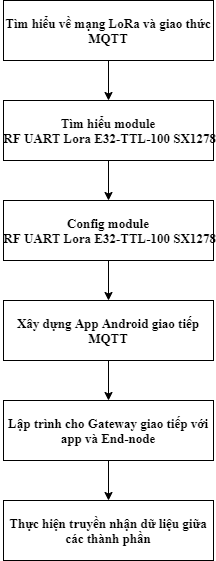
\includegraphics[scale=.5]{Chapter 1/image chapter 1/kehoachthuchien.png}
	\caption[Kế hoạch thực hiện]{Kế hoạch thực hiện}
	\label{hinh11}
\end{figure}


\section*{CHƯƠNG 2: LÝ THUYẾT}
\addcontentsline{toc}{section}{\numberline {} CHƯƠNG 2: LÝ THUYẾT}
\setcounter{section}{2}
\setcounter{subsection}{0}
\subsection{CÔNG NGHỆ LORA}
\subsubsection{Khái niệm}
LoRa là viết tắt của Long Range Radio được nghiên cứu và phát triển bởi Cycleo và sau này được mua lại bởi công ty Semtech năm 2012. Với công nghệ này, chúng ta có thể truyền dữ liệu với khoảng cách lên hàng km mà không cần các mạch khuếch đại công suất; từ đó giúp tiết kiệm năng lượng tiêu thụ khi truyền/nhận dữ liệu. Do đó, LoRa có thể được áp dụng rộng rãi trong các ứng dụng thu thập dữ liệu như sensor network trong đó các sensor node có thể gửi giá trị đo đạc về trung tâm cách xa hàng km và có thể hoạt động với battery trong thời gian dài trước khi cần thay pin.\\
\indent Với tầm xa ,nền tảng không dây công suất thấp là sự lựa chọn công nghệ phổ biến hiện hành để xây dựng mạng iot trên thế giới ứng dụng iot thông minh đã cải thiện theo cách tương tác và giải quết giải quyết một số thách thức lớn nhất mà các thành phố và cộng đồng đang phải đối mặt :biến đổi khí hậu ,kiểm soát ô nhiễm cảnh báo thiên tai và cứu mạng .Kinh doanh cũng được hưởng lợi thông qua cũng như giảm được chi phí
Đây là RF công nghệ không dây được tích hợp vào xe ô tô, đèn đường , sản xuất thiết bị , đồ gia dụng thiết bị đeo được bất cứ điều gì , thực sự . Công nghệ Lora đang làm thế giới ta một hành tinh thông minh\\
\indent Dưới đây là hình ảnh để bạn hiểu rõ nét về tầm xa của Lora:
\begin{figure}[H]
	\centering
	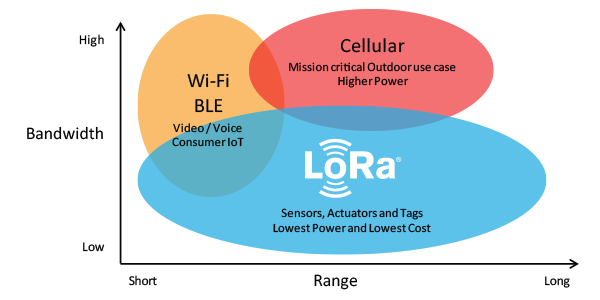
\includegraphics[scale=.5]{Chapter 2/image chapter 2/tamxaLoRa.png}
	\caption[Ảnh minh hoạ tầm xa LoRa]{Ảnh minh hoạ tầm xa LoRa}
	\label{hinh21}
\end{figure}
\subsubsection{Nguyên lý hoạt động}
LoRa sử dụng kỹ thuật điều chế gọi là Chirp Spread Spectrum. Có thể hiểu nôm na nguyên lý này là dữ liệu sẽ được băm bằng các xung cao tần để tạo ra tín hiệu có dãy tần số cao hơn tần số của dữ liệu gốc (cái này gọi là chipped); sau đó tín hiệu cao tần này tiếp tục được mã hoá theo các chuỗi chirp signal (là các tín hiệu hình sin có tần số thay đổi theo thời gian; có 2 loại chirp signal là up-chirp có tần số tăng theo thời gian và down-chirp có tần số giảm theo thời gian; và việc mã hoá theo nguyên tắc bit 1 sẽ sử dụng up-chirp, và bit 0 sẽ sử dụng down-chirp) trước khi truyền ra anten để gửi đi.\\
\indent Theo Semtech công bố thì nguyên lý này giúp giảm độ phức tạp và độ chính xác cần thiết của mạch nhận để có thể giải mã và điều chế lại dữ liệu; hơn nữa LoRa không cần công suất phát lớn mà vẫn có thể truyền xa vì tín hiệu Lora có thể được nhận ở khoảng cách xa ngay cả độ mạnh tín hiệu thấp hơn cả nhiễu môi trường xung quanh.\\
\indent Băng tần làm việc của LoRa từ 430MHz đến 915MHz cho từng khu vực khác nhau trên thế giới:
\begin{itemize}
	\item 430MHz cho châu Á
	\item 780MHz cho Trung Quốc
	\item 433MHz hoặc 866MHz cho châu Âu
	\item 915MHz cho USA
\end{itemize}

\indent Nhờ sử dụng chirp signal mà các tín hiệu LoRa với các chirp rate khác nhau có thể hoạt động trong cùng 1 khu vực mà không gây nhiễu cho nhau. Điều này cho phép nhiều thiết bị LoRa có thể trao đổi dữ liệu trên nhiều kênh đồng thời (mỗi kênh cho 1 chirprate)
\subsubsection{Module thu phát RF UART E32-TTL-100}
\begin{figure}[H]
	\centering
	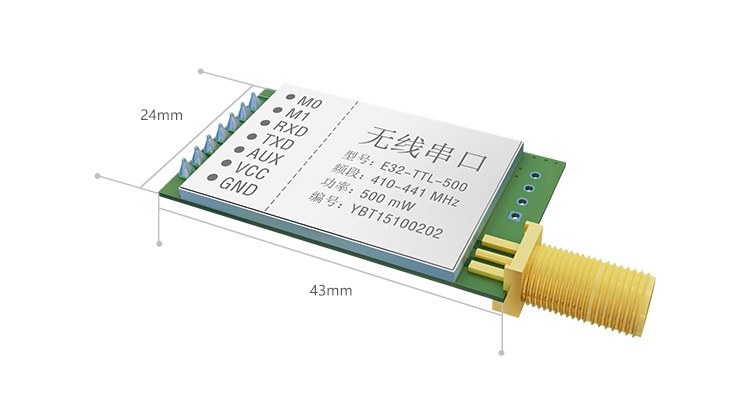
\includegraphics[scale=.4]{Chapter 2/image chapter 2/E32.jpg}
	\caption[Module RF UART E32-TTL-100]{Module RF UART E32-TTL-100}
	\label{hinh22}
\end{figure}
Mạch thu phát RF UART Lora SX1278 433Mhz 3000m sử dụng chip SX1278 của nhà sản xuất SEMTECH chuẩn giao tiếp LORA (Long Range), chuẩn LORA mang đến hai yếu tố quan trọng là tiết kiệm năng lượng và khoảng cách phát siêu xa ( Ultimate long range wireless solution), ngoài ra nó còn có khả năng cấu hình để tạo thành mạng nên hiện tại được phát triển và sử dụng rất nhiều trong các nghiên cứu về IoT.\\
\indent Mạch thu phát RF UART Lora SX1278 433Mhz 3000m được tích hợp phần chuyển đổi giao tiếp SPI của SX1278 sang UART giúp việc giao tiếp và sử dụng rất dễ dàng, chỉ cần kết nối với Software của hãng để cấu hình địa chỉ , tốc độ và công suất truyền là có thể sử dụng.\\
\indent \textbf{Thông số kỹ thuật:}
\begin{itemize}
	\item Model: E32-TTL-100 RF
	\item Điện áp hoạt đông: 2.3 - 5.5 VDC
	\item Điện áp giao tiếp: TTL-3.3V
	\item Giao tiếp UART Data bits 8, Stop bits 1, Parity none, tốc độ từ 1200 - 115200.
	\item Tần số: 410 - 441Mhz
	\item Công suất: 20dbm (100mW)
	\item Khoảng cách truyền tối đa trong điều kiện lý tưởng: 3000m
	\item Tốc độ truyền: 0.3 - 19.2 Kbps ( mặc định 2.4 Kbps)
	\item 512bytes bộ đệm
	\item Hỗ trợ 65536 địa chỉ cấu hình.
	\item Kích thước: 21x36mm.
\end{itemize}
\begin{figure}[H]
	\centering
	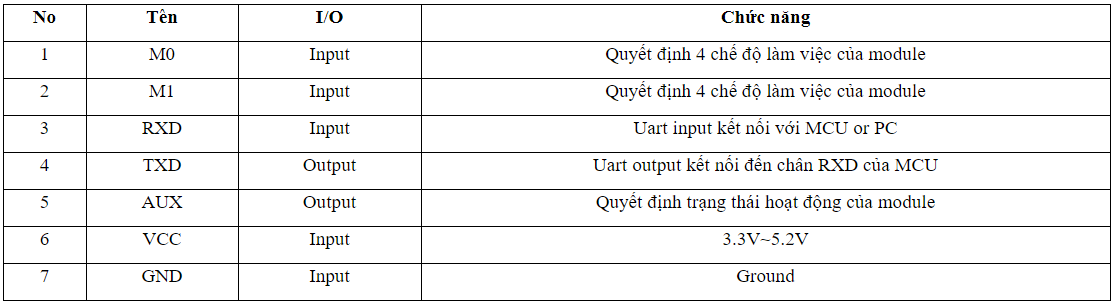
\includegraphics[scale=.5]{Chapter 2/image chapter 2/sodochanvachucnangE32.png}
	\caption[Sơ đồ chân và chức năng của module LoRa E32]{Sơ đồ chân và chức năng của module LoRa E32}
	\label{hinh23}
\end{figure}
\begin{figure}[H]
	\centering
	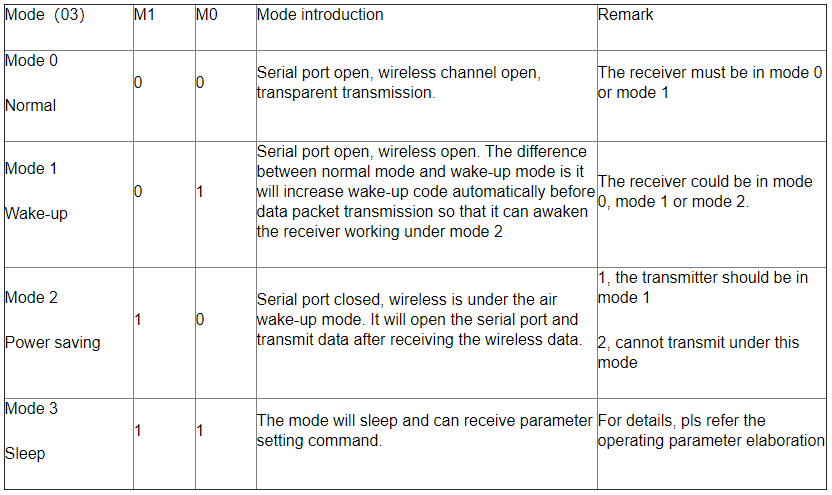
\includegraphics[scale=.5]{Chapter 2/image chapter 2/workmodeE32.png}
	\caption[Chế độ làm việc của module LoRa E32]{Chế độ làm việc của module LoRa E32}
	\label{hinh24}
\end{figure}


\subsection{GIAO THỨC MQTT}
\subsubsection{Khái niệm}
\subsubsection{Nguyên lý hoạt động}


\section*{CHƯƠNG 3: MCU VÀ PHẦN CỨNG ĐƯỢC SỬ DỤNG TRONG THỰC TẬP}
\addcontentsline{toc}{section}{\numberline {} CHƯƠNG 3: MCU VÀ PHẦN CỨNG ĐƯỢC SỬ DỤNG TRONG THỰC TẬP}
\setcounter{section}{3}
\setcounter{subsection}{0}
\subsection{ARDUINO NANO}
\subsection{RASPBERRY PI 3}
\subsection{MODULE RF UART E32-TTL-100}
\subsection{DHT22 TEMPERATURE AND HUMIDITY SENSOR}
\subsection{MODULE 2 RELAY OPTO 5VDC}

\section*{CHƯƠNG 4: KẾT QUẢ THỰC HIỆN}
\addcontentsline{toc}{section}{\numberline {} CHƯƠNG 4: KẾT QUẢ THỰC HIỆN}
\setcounter{section}{4}
\setcounter{figure}{0}
\setcounter{subsection}{0}
\subsection{KẾT QUẢ THI CÔNG PHẦN CỨNG}
\begin{figure}[H]
	\centering
	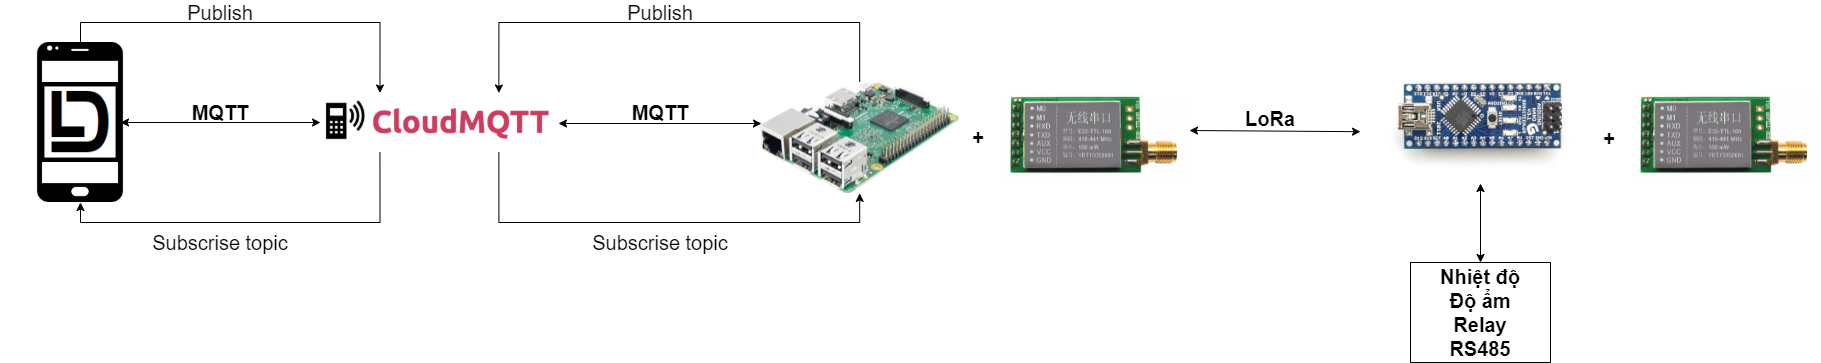
\includegraphics[scale=0.2]{Chapter 4/image chapter 4/figure.png}
	\caption[Sơ đồ các giao tiếp phần cứng]{Sơ đồ các giao tiếp phần cứng}
	\label{hinh41}
\end{figure}
\begin{figure}[H]
	\centering
	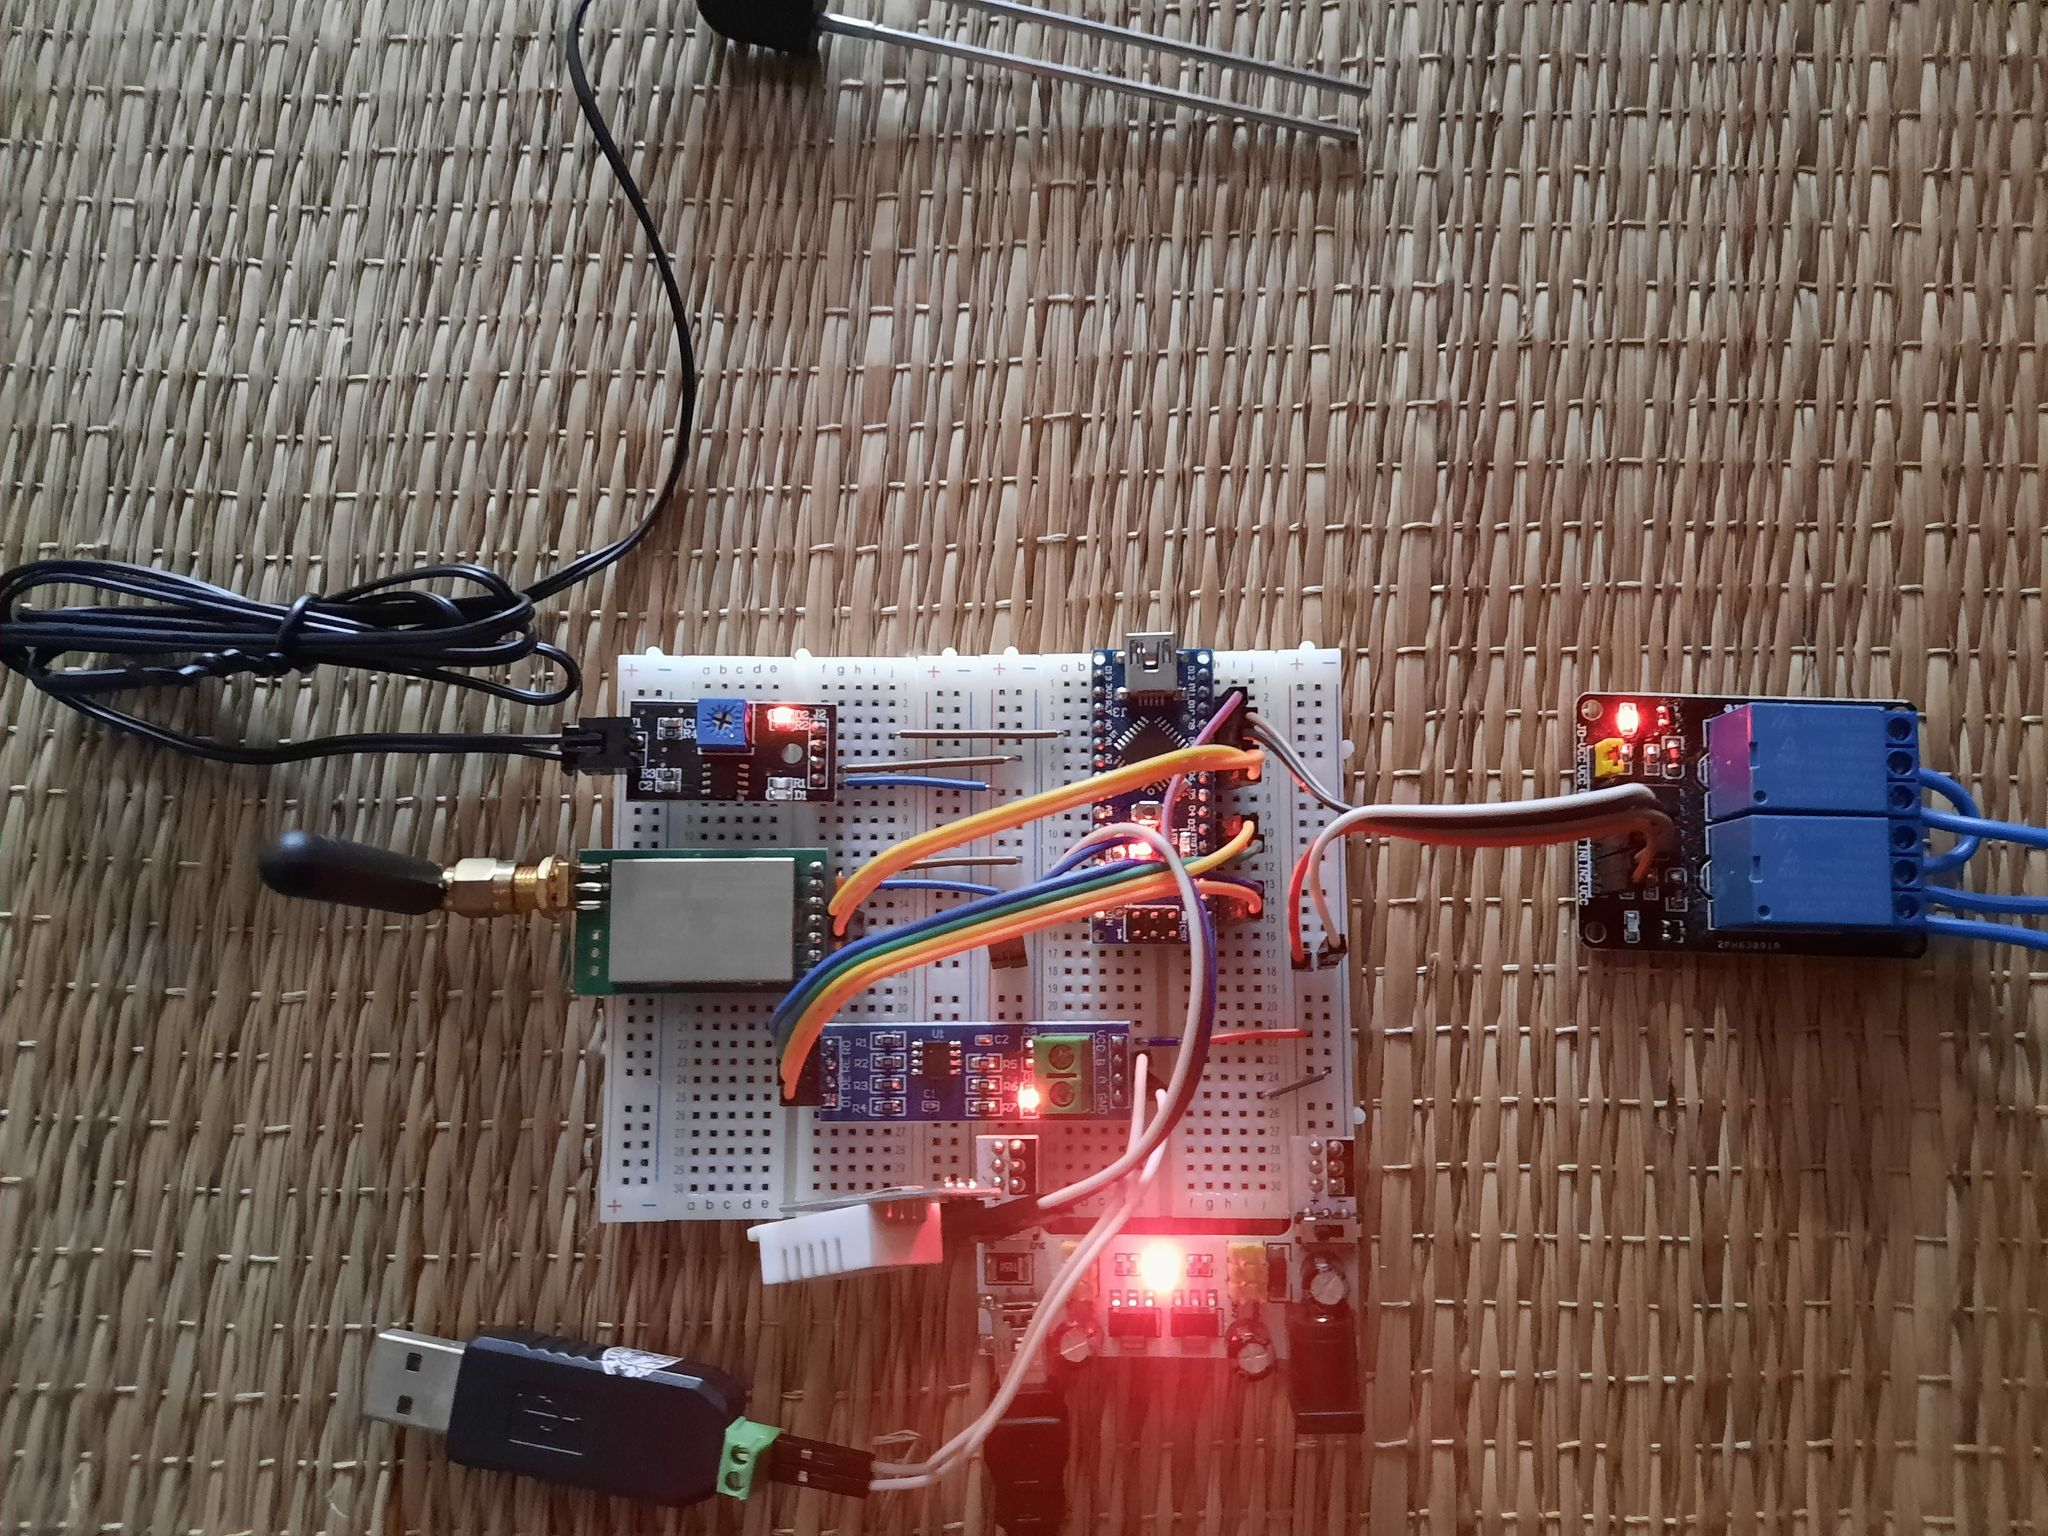
\includegraphics[scale=0.2]{Chapter 4/image chapter 4/phancung.jpg}
	\caption[Phần cứng end-Node trong thực tế]{Phần cứng end-Node trong thực tế}
	\label{hinh42}
\end{figure}
\subsection{KIỂM TRA ĐỘ CHÍNH XÁC THÔNG SỐ NHIỆT ĐỘ \& ĐỘ ẨM}
\subsection{KIỂM TRA HOẠT ĐỘNG CỦA MODULE 2 RELAY}

\section*{CHƯƠNG 5: KẾT LUẬN VÀ HƯỚNG PHÁT TRIỂN}
\addcontentsline{toc}{section}{\numberline {} CHƯƠNG 5: KẾT LUẬN VÀ HƯỚNG PHÁT TRIỂN}
\setcounter{section}{5}
\setcounter{subsection}{0}
\subsection{KẾT LUẬN}
\subsection{HƯỚNG PHÁT TRIỂN}



\end{document}
